\documentclass{article}
\usepackage{blindtext}
\usepackage[a4paper, total={6in, 9.4in}]{geometry}
\usepackage{indentfirst}
\usepackage{wrapfig}
\usepackage{graphicx}
\usepackage{mathtext}
\usepackage{amsmath}
\usepackage{siunitx} % Required for alignment
\usepackage{subfigure}
\usepackage{multirow}
\usepackage{rotating}
\usepackage{afterpage}
\usepackage[T1,T2A]{fontenc}
\usepackage[russian]{babel}
\usepackage{caption}
\usepackage[arrowdel]{physics}
\usepackage{booktabs}

\graphicspath{{pictures/}}

\title{\begin{center}Лабораторная работа №4.7.2\end{center}
Эффект Поккельса}
\author{Севастьян Черняков и Алексей Нистюк}
\date{\today}

\begin{document}

\pagenumbering{gobble}
\maketitle
\pagenumbering{arabic}

\textbf{Цель работы:} Исследовать интерференцию рассеянного света, прошедшего кристалл; наблюдать изменение характера поляризации света при наложении на кристалл электрического поля.

\section{Теоретическая часть}
\subsection{Интерференционные кольца при прохождении света через одноосный кристалл}
\begin{figure}[h]
    \center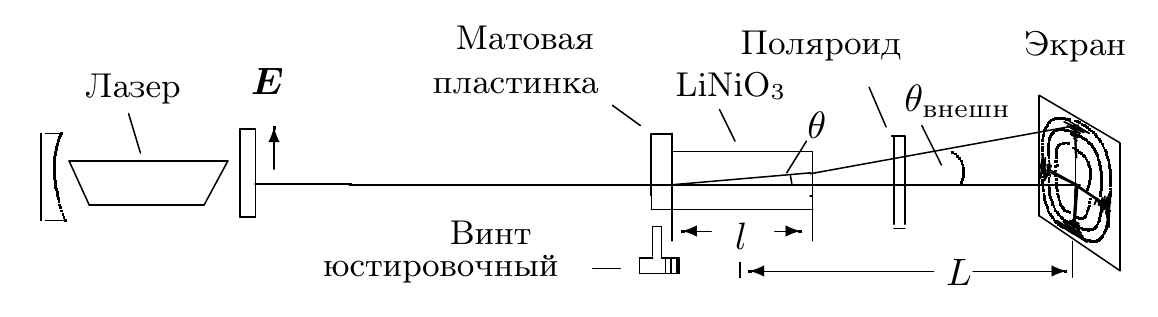
\includegraphics[width = 0.8\linewidth]{ustanovka_kolca.png}
    \caption{Схема для наблюдения интерференционной картины}\label{fig:ustanovka_kolca}
\end{figure}

При прохождении света через одноосный кристалл, показатель преломления необыкновенной
волны зависит от угла между направлением распространения волны и осью кристалла
по формуле

\begin{equation}
    \frac{1}{n_2^2} = \frac{\cos^2 \theta}{n_o^2} + \frac{\sin^2 \theta}{n_e^2}
    \label{eq:pokazatel_prelomlenia}
\end{equation}

Если считать, что $(n_o - n_e) \ll n_o$, то при малых углах $\theta$ можно
воспользоваться приближенной формулой

\begin{equation}
    n_2 \approx n_o - (n_o - n_e) \theta^2
    \label{eq:pokazatel_prelomlenia_approx}
\end{equation}

Показатель преломления обыкновенного луча не зависит от направления распространения:
$n_1 = n_o$. Если длине кристалла $l$, то после прохождения через кристалл между
обыкновенным и необыкновенным лучом набегает разность фаз

\begin{equation}
    \Delta \varphi = \frac{2\pi}{\lambda} l (n_1 - n_2) \approx
    \frac{2\pi}{\lambda} l (n_o - n_e) \theta^2
    \label{eq:raznost_faz}
\end{equation}

Для случая, когда разрешенное направление анализатора перпендикулярно направлению
поляризации лазера, условием для темного кольца с номером $m$ является
$\varphi = 2\pi m$, откуда следует

\begin{equation}
    \theta_m^2 = \frac{\lambda m}{l(n_o - n_e)}
    \label{eq:theta_m}
\end{equation}

При выхоже из кристалла луч преломляется на границе кристалл-воздух, поэтому угол
$\theta_{внешн} \approx n_o \theta$. Радиус $m$-го темного кольца
$r_m = L\theta_{внешн, m}$. Для квадрата радиуса

\begin{equation}
    r_m^2 = \frac{\lambda}{l} \frac{{(n_o L)}^2}{(n_o - n_e)} m
    \label{eq:r_m}
\end{equation}

\subsection{Эффект Поккельса}

\begin{wrapfigure}{l}{0.4\textwidth}
  \begin{center}
    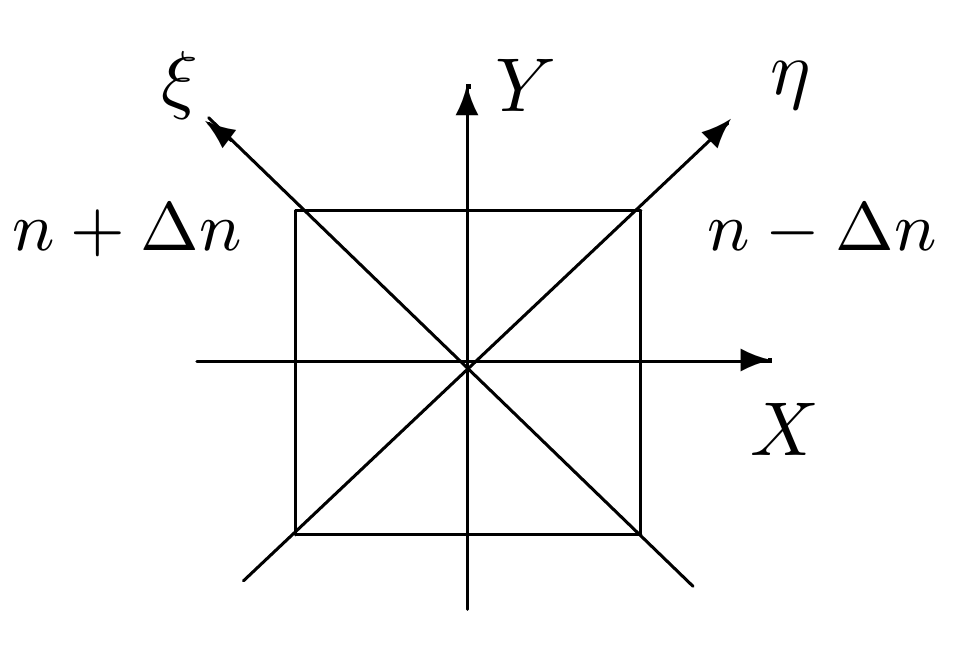
\includegraphics[width=0.38\textwidth]{pokkels_axes.png}
  \end{center}
  \caption{Главные оси при наличии напряжения вдоль $x$}\label{fig:pokkels_axes}
\end{wrapfigure}

При наличии электрического поля вдоль $x$ в кристалле появляются новые перпендикулярные
главные направления, показатели преломления которых равны $n_o \pm \Delta n$, где
$\Delta n = A \cdot E_{x}$. Пусть поляризация лазера вертикальна, а разрешенное
направление анализатора горизонтальна. Тогда, интенсивность света на выходе
будет зависеть от прикладываемого напряжения ($U = E_x d$) по закону

\begin{equation}
    I = I_0 \sin^2\left(\frac{\pi}{2}\frac{U}{U_{\lambda/2}}\right)
    \label{eq:pokkels}
\end{equation}

где
\begin{equation}
    U_{\lambda/2} = \frac{\lambda}{4A} \frac{d}{l}
    \label{eq:poluvolnovoe_napryajenie}
\end{equation}

\vspace{1cm}
\section{Измерения}
\subsection{Интерференционные кольца}

\begin{table}[h]
\begin{center}
\begin{tabular}{|c|c|}
\hline
 № кольца &  r, мм \\
\hline
 1 & 16 \\  \hline
 2 & 26 \\ \hline
 3 & 38 \\ \hline
 4 & 46 \\ \hline
 5 & 54 \\ \hline
 6 & 60 \\ \hline


 
\end{tabular}

$\sigma_r$ = 2мм
\caption{Зависимость радиусов темных колец от номера колец}
\end{center}
\end{table}


\begin{figure}[h!]
    \center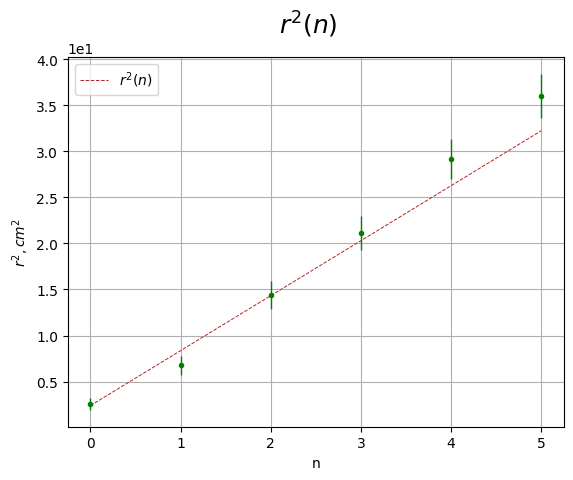
\includegraphics[width = 0.9\linewidth]{graph.png}
    \caption{Линеаризованные график зависимости радиуса колец от номера}\label{fig:r_m}
\end{figure}

Из графика (метод взвешенных наименьших квадратов) и согласно формуле (\ref{eq:r_m})

\begin{equation*}
    \frac{\lambda}{l} \frac{{(n_o L)}^2}{(n_o - n_e)} = (5.97 \pm 0.24) \text{ см}^2
\end{equation*}

Для нашей установки $\lambda = 6328$ \AA, $l = 26$ мм, $L = (76.0 \pm 0.5)$ см,
$n_o = 2.29$. После подстановки получаем

\begin{equation}
    n_o - n_e = (0.081 \pm 0.003)
\end{equation}
\newpage
\subsection{Эффект Поккельса}
\begin{wrapfigure}{L}{0.5\textwidth}
    \begin{center}
      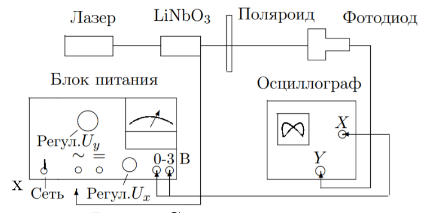
\includegraphics[width=0.4\textwidth]{image.png}
    \end{center}
    \caption{схема установки}
\end{wrapfigure}
Соберем установку по рис.4, определим полуволновое напряжение по разности 
напряжений при максимуме и минимуме у фигуры Лиссажу:

$U_{\lambda/2} = (420 \pm 15)$В

подав на кристалл $U_{\lambda/4} = \dfrac{U_{\lambda/2}}{2}$, убеждаемся, что поляризация круговая, при вращении анализатора интенсивность не изменяется


\vspace{20pt}
\begin{figure}[h!]
    \begin{center}
        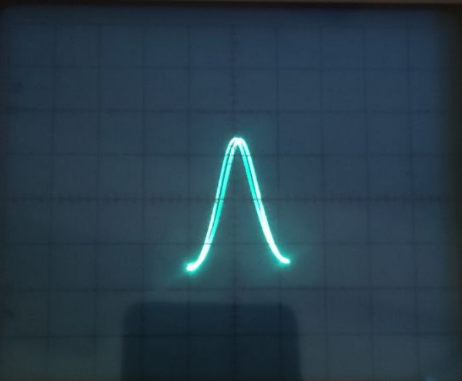
\includegraphics[width = 0.3\linewidth]{1.png}
        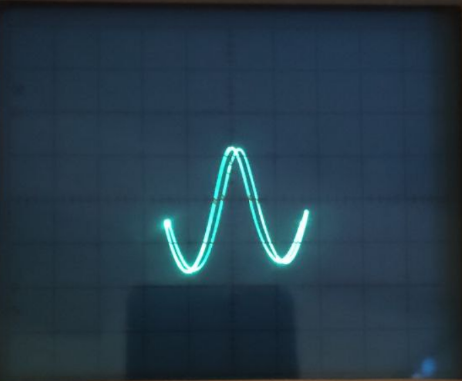
\includegraphics[width = 0.3\linewidth]{2.png}
        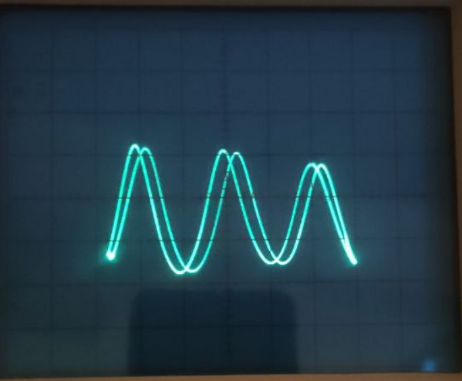
\includegraphics[width = 0.3\linewidth]{3.png}
    \end{center}
    \caption{Фигуры лиссажу для U$_{\lambda/2}$, U$_{\lambda}$ и U$_{3\lambda/2}$}
\end{figure}

.

.
\section{Вывод} 
В работе с помощью интерференционной картины было определено двулучепреломления ниобата лития (по угловому коэффициенту зависимости квадрата радиуса тёмного пятна от номера тёмного пятна с помощью формулы 2).

В открытых источниках удалось найти информацию о табличном значении

$\Delta n = 0.083$, 

что совпало с учетом погрешности с полученным значением 

$n_o - n_e = (0.081 \pm 0.003)$

Также был исследован эффект Поккельса и полуволновое напряжение - с помощью наблюдения изменения интенсивности и с помощью фигур Лиссажу, полученное значение было дополнительно проверено экспериментально: при напряжении $U_{\lambda/4}$ была получена круговая поляризация. 



\end{document}